\documentclass[11pt,a4paper]{article}
\usepackage[latin1]{inputenc}
\usepackage[dutch]{babel}
\usepackage{amsmath}
\usepackage{amsfonts}
\usepackage{pgfplots} % LaTeX
\usepackage{amssymb}
\author{Mathias Dekempeneer}
\begin{document}

\begin{figure}[!h]
\centering
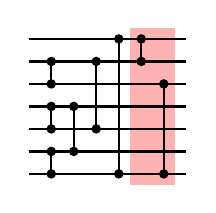
\begin{tikzpicture}
\def\x{3.5}
\fill [red!30] (4.5/\x,0.5/\x) -- (6.5/\x,0.5/\x) -- (6.5/\x,7.5/\x) -- (4.5/\x,7.5/\x) -- cycle;
\foreach \a in {1/\x, 2/\x, 3/\x, 4/\x, 5/\x, 6/\x, 7/\x}
  \draw[thick] (0,\a) -- ++(7/\x,0);
\foreach \b in {{1/\x,1/\x},{1/\x,2/\x},{1/\x,3/\x},{1/\x,4/\x},{1/\x,5/\x},{1/\x,6/\x},{2/\x,2/\x},{2/\x,4/\x},{3/\x,3/\x},{3/\x,6/\x},{4/\x,1/\x},{4/\x,7/\x},{5/\x,6/\x},{5/\x,7/\x},{6/\x,1/\x},{6/\x,5/\x}}
  \filldraw (\b) circle (1.5 pt);
\draw[thick] (1/\x,1/\x) -- (1/\x,2/\x);
\draw[thick] (1/\x,3/\x) -- (1/\x,4/\x);
\draw[thick] (1/\x,5/\x) -- (1/\x,6/\x);
\draw[thick] (2/\x,2/\x) -- (2/\x,4/\x);
\draw[thick] (3/\x,3/\x) -- (3/\x,6/\x);
\draw[thick] (4/\x,1/\x) -- (4/\x,7/\x);
\draw[thick] (5/\x,6/\x) -- (5/\x,7/\x);
\draw[thick] (6/\x,1/\x) -- (6/\x,5/\x);
\end{tikzpicture}
\caption{Sorteernetwerk 9 kanalen, 25 comparatoren}
\end{figure}

\begin{figure}[!h]
\centering
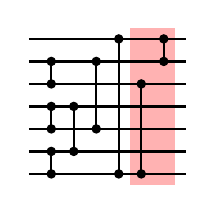
\begin{tikzpicture}
\def\x{3.5}
\fill [red!30] (4.5/\x,0.5/\x) -- (6.5/\x,0.5/\x) -- (6.5/\x,7.5/\x) -- (4.5/\x,7.5/\x) -- cycle;
\foreach \a in {1/\x, 2/\x, 3/\x, 4/\x, 5/\x, 6/\x, 7/\x}
  \draw[thick] (0,\a) -- ++(7/\x,0);
\foreach \b in {{1/\x,1/\x},{1/\x,2/\x},{1/\x,3/\x},{1/\x,4/\x},{1/\x,5/\x},{1/\x,6/\x},{2/\x,2/\x},{2/\x,4/\x},{3/\x,3/\x},{3/\x,6/\x},{4/\x,1/\x},{4/\x,7/\x},{6/\x,6/\x},{6/\x,7/\x},{5/\x,1/\x},{5/\x,5/\x}}
  \filldraw (\b) circle (1.5 pt);
\draw[thick] (1/\x,1/\x) -- (1/\x,2/\x);
\draw[thick] (1/\x,3/\x) -- (1/\x,4/\x);
\draw[thick] (1/\x,5/\x) -- (1/\x,6/\x);
\draw[thick] (2/\x,2/\x) -- (2/\x,4/\x);
\draw[thick] (3/\x,3/\x) -- (3/\x,6/\x);
\draw[thick] (4/\x,1/\x) -- (4/\x,7/\x);
\draw[thick] (6/\x,6/\x) -- (6/\x,7/\x);
\draw[thick] (5/\x,1/\x) -- (5/\x,5/\x);
\end{tikzpicture}
\caption{Sorteernetwerk 9 kanalen, 25 comparatoren}
\end{figure}

\begin{figure}[!h]
\centering
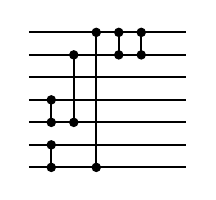
\begin{tikzpicture}
%\fill [gray!15] (1.5,1.5) -- (2.5,1.5) -- (2.5,2.5) -- (1.5,2.5) -- cycle;
%\foreach \a in {1,..,9}
\def\x{3.5}
\foreach \a in {1/\x, 2/\x, 3/\x, 4/\x, 5/\x, 6/\x, 7/\x}
  \draw[thick] (0,\a) -- ++(7/\x,0);
\foreach \b in {{1/\x,1/\x},{1/\x,2/\x},{1/\x,3/\x},{1/\x,4/\x},{2/\x,3/\x},{2/\x,6/\x},{3/\x,1/\x},{3/\x,7/\x},{4/\x,6/\x},{4/\x,7/\x},{5/\x,6/\x},{5/\x,7/\x}}
  \filldraw (\b) circle (1.5 pt);
\draw[thick] (1/\x,1/\x) -- (1/\x,2/\x);
\draw[thick] (1/\x,3/\x) -- (1/\x,4/\x);
\draw[thick] (2/\x,3/\x) -- (2/\x,6/\x);
\draw[thick] (3/\x,1/\x) -- (3/\x,7/\x);
\draw[thick] (4/\x,6/\x) -- (4/\x,7/\x);
\draw[thick] (5/\x,6/\x) -- (5/\x,7/\x);
\end{tikzpicture}
\caption{Sorteernetwerk 9 kanalen, 25 comparatoren}
\end{figure}

\end{document}